%%%%%%%%%%%%%%%%%%%%%%%%%%%%%%%%%%%%%%%%%
% Arsclassica Article
% LaTeX Template
% Version 1.1 (1/8/17)
%
% This template has been downloaded from:
% http://www.LaTeXTemplates.com
%
% Original author:
% Lorenzo Pantieri (http://www.lorenzopantieri.net) with extensive modifications by:
% Vel (vel@latextemplates.com)
%
% License:
% CC BY-NC-SA 3.0 (http://creativecommons.org/licenses/by-nc-sa/3.0/)
%
%%%%%%%%%%%%%%%%%%%%%%%%%%%%%%%%%%%%%%%%%

%----------------------------------------------------------------------------------------
%	PACKAGES AND OTHER DOCUMENT CONFIGURATIONS
%----------------------------------------------------------------------------------------

\documentclass[
10pt, % Main document font size
a4paper, % Paper type, use 'letterpaper' for US Letter paper
oneside, % One page layout (no page indentation)
%twoside, % Two page layout (page indentation for binding and different headers)
headinclude,footinclude, % Extra spacing for the header and footer
BCOR5mm, % Binding correction
]{scrartcl}

%%%%%%%%%%%%%%%%%%%%%%%%%%%%%%%%%%%%%%%%%
% Arsclassica Article
% Structure Specification File
%
% This file has been downloaded from:
% http://www.LaTeXTemplates.com
%
% Original author:
% Lorenzo Pantieri (http://www.lorenzopantieri.net) with extensive modifications by:
% Vel (vel@latextemplates.com)
%
% License:
% CC BY-NC-SA 3.0 (http://creativecommons.org/licenses/by-nc-sa/3.0/)
%
%%%%%%%%%%%%%%%%%%%%%%%%%%%%%%%%%%%%%%%%%

%----------------------------------------------------------------------------------------
%	REQUIRED PACKAGES
%----------------------------------------------------------------------------------------

\usepackage[
nochapters, % Turn off chapters since this is an article        
beramono, % Use the Bera Mono font for monospaced text (\texttt)
eulermath,% Use the Euler font for mathematics
pdfspacing, % Makes use of pdftex’ letter spacing capabilities via the microtype package
dottedtoc % Dotted lines leading to the page numbers in the table of contents
]{classicthesis} % The layout is based on the Classic Thesis style

\usepackage{arsclassica} % Modifies the Classic Thesis package

\usepackage[T1]{fontenc} % Use 8-bit encoding that has 256 glyphs

\usepackage[utf8]{inputenc} % Required for including letters with accents

\usepackage{graphicx} % Required for including images
\graphicspath{{Figures/}} % Set the default folder for images

\usepackage{enumitem} % Required for manipulating the whitespace between and within lists

\usepackage{lipsum} % Used for inserting dummy 'Lorem ipsum' text into the template

\usepackage{subfig} % Required for creating figures with multiple parts (subfigures)

\usepackage{amsmath,amssymb,amsthm} % For including math equations, theorems, symbols, etc

\usepackage{varioref} % More descriptive referencing

%----------------------------------------------------------------------------------------
%	THEOREM STYLES
%---------------------------------------------------------------------------------------

\theoremstyle{definition} % Define theorem styles here based on the definition style (used for definitions and examples)
\newtheorem{definition}{Definition}

\theoremstyle{plain} % Define theorem styles here based on the plain style (used for theorems, lemmas, propositions)
\newtheorem{theorem}{Theorem}

\theoremstyle{remark} % Define theorem styles here based on the remark style (used for remarks and notes)

%----------------------------------------------------------------------------------------
%	HYPERLINKS
%---------------------------------------------------------------------------------------

\hypersetup{
%draft, % Uncomment to remove all links (useful for printing in black and white)
colorlinks=true, breaklinks=true, bookmarks=true,bookmarksnumbered,
urlcolor=webbrown, linkcolor=RoyalBlue, citecolor=webgreen, % Link colors
pdftitle={}, % PDF title
pdfauthor={\textcopyright}, % PDF Author
pdfsubject={}, % PDF Subject
pdfkeywords={}, % PDF Keywords
pdfcreator={pdfLaTeX}, % PDF Creator
pdfproducer={LaTeX with hyperref and ClassicThesis} % PDF producer
} % Include the structure.tex file which specified the document structure and layout

\hyphenation{Fortran hy-phen-ation} % Specify custom hyphenation points in words with dashes where you would like hyphenation to occur, or alternatively, don't put any dashes in a word to stop hyphenation altogether

%----------------------------------------------------------------------------------------
%	TITLE AND AUTHOR(S)
%----------------------------------------------------------------------------------------

\title{\normalfont\spacedallcaps{Non-Negative Matrix Factorization and Applications}} % The article title

\author{\spacedlowsmallcaps{Piper Morris, Brandon Bonifas-Reyes \& Rad Mallari\textsuperscript{1}}} % The article author(s) - author affiliations need to be specified in the AUTHOR AFFILIATIONS block

%----------------------------------------------------------------------------------------

\begin{document}

%----------------------------------------------------------------------------------------
%	HEADERS
%----------------------------------------------------------------------------------------

\renewcommand{\sectionmark}[1]{\markright{\spacedlowsmallcaps{#1}}} % The header for all pages (oneside) or for even pages (twoside)
\lehead{\mbox{\llap{\small\thepage\kern1em\color{halfgray} \vline}\color{halfgray}\hspace{0.5em}\rightmark\hfil}} % The header style

\pagestyle{scrheadings} % Enable the headers specified in this block

%----------------------------------------------------------------------------------------
%	TABLE OF CONTENTS & LISTS OF FIGURES AND TABLES
%----------------------------------------------------------------------------------------

\maketitle % Print the title/author/date block
\setcounter{tocdepth}{2} % Set the depth of the table of contents to show sections and subsections only
\tableofcontents % Print the table of contents
\listoffigures % Print the list of figures
\newpage
%----------------------------------------------------------------------------------------
%	ABSTRACT
%----------------------------------------------------------------------------------------

\section*{Abstract} % This section will not appear in the table of contents due to the star (\section*)
\textbf{Non-negative matrix factorization}, often referred to as NMF, is one of many unsupervised learning algorithms used to extract significant figures from large sets of data. It is a relatively new process that has become an important tool in dimensionality reduction, and is comparable to other factorization techniques such as \textbf{principal component analysis} (PCA) and \textbf{vector quantification} (VQ). NMF is unique due to its constraint on non-negative elements resulting in an often preferable outcome. NMF has garnered popularity in machine-learning industries because the algorithm is able to efficiently extract sparse data and provide respective factors that one can easily interpret.

%----------------------------------------------------------------------------------------
%	AUTHOR AFFILIATIONS
%----------------------------------------------------------------------------------------

\let\thefootnote\relax\footnotetext{\textsuperscript{1} \textit{Department of Mathematics, University of California, Santa Barbara}}

%----------------------------------------------------------------------------------------

%----------------------------------------------------------------------------------------
%	INTRODUCTION
%----------------------------------------------------------------------------------------

\section{Introduction}

A statement requiring citation \cite{Figueredo:2009dg}.

Given an $n\times m$ non-negative matrix $A$, NMF aims to express $A$ as two similarly non-negative matrices of smaller dimensions, $W$ and $H$. Note that when referring to a non-negative matrix, we are discussing a matrix in which all its entries are real and greater than or equal to zero. $W$ is an $m\times k$ matrix consisting of $k$ \textit{basis elements} of $A$ and $H$ is a $k\times n$ matrix consisting of the coefficients, or \textit{weights}, related to the entries of $W$. We denote some $r>0$ as the inner dimension of $W$ and $H$ and the smallest such instance where $r$ holds is called the \emph{factorization rank}. Because our resulting NMF is a nonnegative approximation, $W,H$ (holding the same properties) may not be unique either. Nonetheless, we utilize methods for measuring the error of our approximations.

%----------------------------------------------------------------------------------------
%	COST FUNCTIONS
%----------------------------------------------------------------------------------------

\section{Cost Functions}
As mentioned above, the reason NMF is so complex is because its algorithms attempt to replicate the original matrix, namely $A$. Thus, the product of $WH$ will be a representation of $A$, and not an exact replica. As a result, we implement various methods to go about solving an NMF problem. One of the most common ways to execute this is by using a cost function, of which there are several. Cost functions share a common goal of attempting to minimize the error between our original matrix and the product of our factorization.
One useful method is accomplished by minimizing the square of the Euclidean distance,  which is often referred to as minimizing the Frobenius norm as it relates specifically to matrices. See the Frobenius norm below:
$$\lVert A-WH\rVert^{2}_{F}=\sum_{ij}(A-WH)_{ij}$$
This measure is often chosen because it is not as expensive as other cost functions in terms of calculation. Additionally, it has a key property in that it remains invariant under rotations/orthogonal transformations. Secondly, it accounts for the presence of Gaussian noise and is recognized as the Euclidean norm because it compiles all the rows/columns of a matrix and concatenates them to produce one vector.  While applying the frobenius norm, iterative update rules are used to exchange a randomized WH matrix with one that has a smaller error. We continue to do this until the error meets a predetermined requirement.
An alternative norm used in the process of decomposition is the Kullback Liebler divergence:
% cite this
$$D_{KL}(A\vert WH):=\sum_{i=1}^{m}\sum_{j=1}^{n}((WH)_{ij}-A_{ij}\log(WH)_{ij})+\sum_{i=1}^{m}\sum_{j=1}^{n}(A_{ij}\log A_{ij}-A_{ij})$$

% needs more explanation

%----------------------------------------------------------------------------------------
%	MULTIPLICATIVE UPDATE RULE
%----------------------------------------------------------------------------------------

\section{Multiplicative Update Rule}

% cite this (Use Lee and Seung's paper??)
A common approach to NMF problems is Lee and Seung's multiplicative update rule. The multiplicative update rule became popular due to its simplicity, however, it is criticized for its slow convergence and lack of guarantee of convergence to a stationary point, which is necessary to find a local minimum.
% cite this
The Formula is given by:
$$W\leftarrow W\cdot\frac{(VH^{T})}{(WHH^{T})}$$
$$H\leftarrow H\cdot\frac{(W^{T}V)}{W^{T}WH}$$
%------------------------------------------------


%----------------------------------------------------------------------------------------
%	APPLICATIONS
%----------------------------------------------------------------------------------------
\section{Applications}

% add images of python code?
We created an application of NMF which decomposes an image matrix, then returns $W$, $H$, and the resulting $WH$ which then is plotted and shown. Since $WH$ and are not exact, we see that the image return is only approximately the original image~\vref{fig:application}. The script\textsuperscript{2} is written using Python, and deploys the multiplicative update rule to iterate until the error between the original matrix $A$ and $W,H$ are less than a specified error or a specified number of iterations. From here we can talk about implications of these results:

\let\thefootnote\relax\footnotetext{\textsuperscript{2} \url{https://github.com/radimallari/108C_Final_Project}}

\subsection{Facial Recognition}
Assuming we have a collection of the same face, we can flatten each image to a single vector and this would be our training set, denoting it by $X_{1},X_{2},...,X_{n}$ respectively. The collection of these flattened images could be written as matrix $X$, i.e.
$$X=\begin{bmatrix}
        \vdots & \vdots &       & \vdots \\
        X_{1}  & X_{2}  & \dots & X_{N}  \\
        \vdots & \vdots &       & \vdots
    \end{bmatrix}$$
By applying NMF to this matrix, we have $X=WH$, we can identify prominent features on the face with the $W$ matrix and their weights with $H$. By taking an image matrix outside of the set, then applying NMF, say $X'=W'H'$, we can use the result of the training data to find the best fit of $W'H'$, in otherwords, a rough estimation on who the new image matrix is.
\subsection{Image Processing}
NMF often begins its canonical relationship with the real world in the field of image processing. We take a simple image of a face with p pixels, and reduce the dimensions of the data to a single vector such that the ith entry represents the ith pixel. Then we can allow the rows of our matrix A to represent the p pixels and n columns respectively output one image. The process of NMF, as we have defined it, will produce W and H to be multiplied, where the columns of W embody the basis images and H gives instruction on how to sum up the aforementioned images. All this to reconstruct an approximation of the originally provided face (See Figure~\vref{fig:facedecomp}).

\subsection{Text Mining}
We utilize NMF in the field of topic recovery/document classification.
Let each column of A correspond to a text and each row relate to a keyword.
Construct every $(i,j)$-th entry in such a way where it represents every time a given word $(i)$ comes up in a document $(j)$.
%needs citation
This is a type of quality of term frequency construction in such a model, namely the bag-of-words model, where each document being analyzed has its respective set of words.
The ordering of words here is not accounted for.
The concept of sparseness appears once more in A due to the nature of texts/documents which only use a portion of the dictionary.
In any case, NMF provides a decomposition of rank r as follows:
%needs citation
$$A(i,j)\approx\sum_{k=1}^{r}W(i,k)\cdot\sum H(k,j)$$
Note that in the above $A$ is our $j$-th document, $W$ our $k$-th topic, and $H$ conveys the relevance of a topic in a given document.

\begin{figure}[tb]
    \centering
    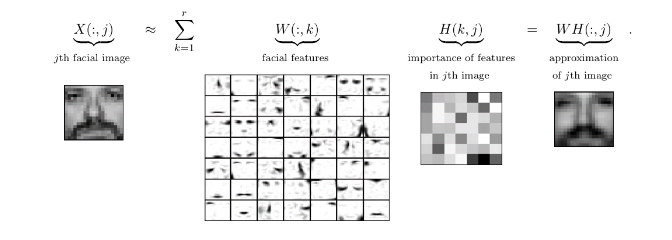
\includegraphics[width=0.7\columnwidth]{Decomposition of face.png}
    \caption[Face Decomposition Using NMF]{Face decomposition with k = 49. \cite{colyer_2019}}
    \label{fig:facedecomp}
\end{figure}

\begin{figure}[tb]
    \centering
    \subfloat[Pre NMF image.]{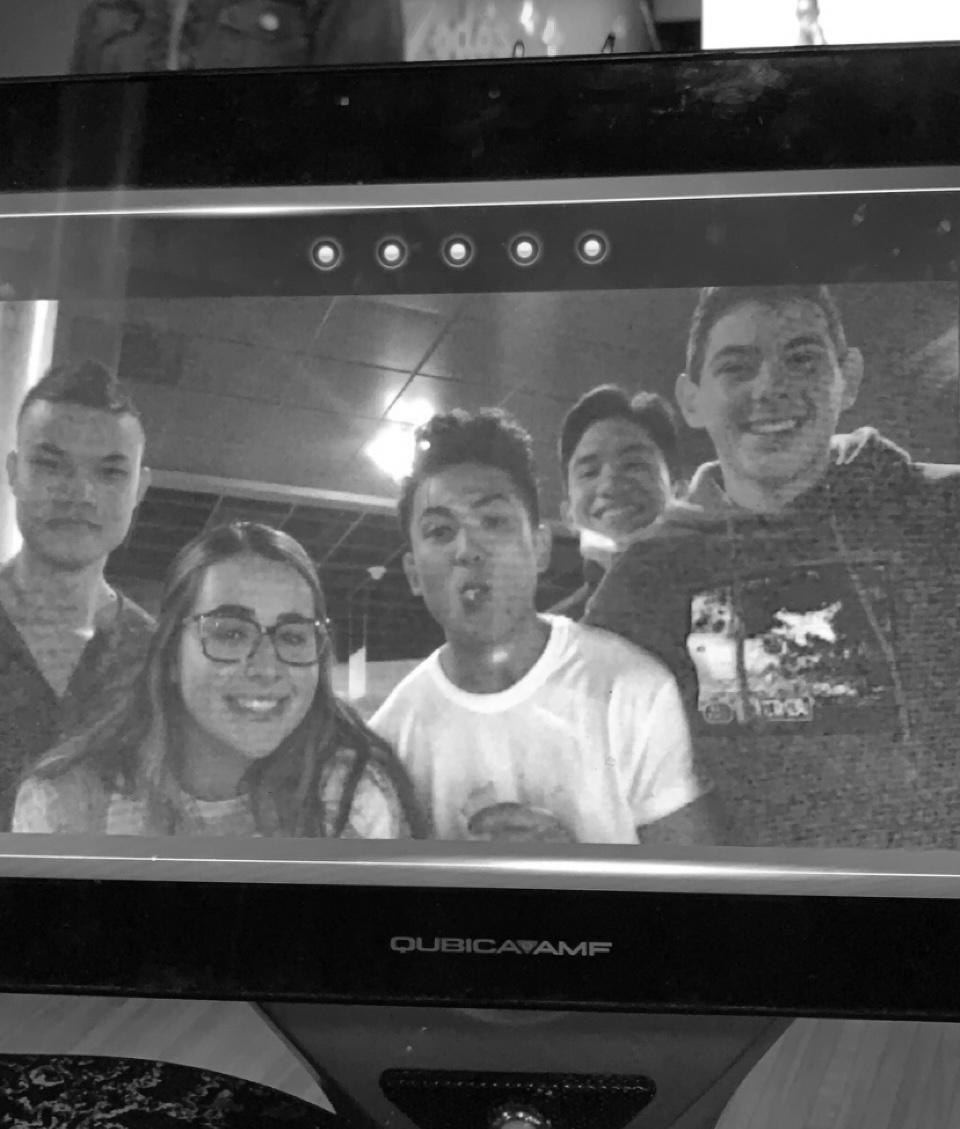
\includegraphics[width=0.5\columnwidth]{preprocessed}}
    \subfloat[Post NMF k = 35.]{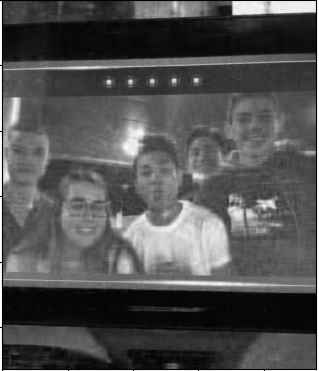
\includegraphics[width=0.5\columnwidth]{NMFk35}}
    \caption{Result of NMF}
    \label{fig:application}
\end{figure}
% ------------------------------------------------
% \subsection{Subsection}

% \lipsum[11] % Dummy text

% \subsubsection{Subsubsection}

% \lipsum[12] % Dummy text

% \begin{description}
% \item[Word] Definition
% \item[Concept] Explanation
% \item[Idea] Text
% \end{description}

% \lipsum[12] % Dummy text

% \begin{itemize}[noitemsep] % [noitemsep] removes whitespace between the items for a compact look
% \item First item in a list
% \item Second item in a list
% \item Third item in a list
% \end{itemize}

% \subsubsection{Table}

% \lipsum[13] % Dummy text

% \begin{table}[hbt]
% \caption{Table of Grades}
% \centering
% \begin{tabular}{llr}
% \toprule
% \multicolumn{2}{c}{Name} \\
% \cmidrule(r){1-2}
% First name & Last Name & Grade \\
% \midrule
% John & Doe & $7.5$ \\
% Richard & Miles & $2$ \\
% \bottomrule
% \end{tabular}
% \label{tab:label}
% \end{table}

% Reference to Table~\vref{tab:label}. % The \vref command specifies the location of the reference

% ------------------------------------------------

% \subsection{Figure Composed of Subfigures}

% Reference the figure composed of multiple subfigures as Figure~\vref{fig:esempio}. Reference one of the subfigures as Figure~\vref{fig:ipsum}. % The \vref command specifies the location of the reference

% \lipsum[15-18] % Dummy text

% \begin{figure}[tb]
% \centering
% \subfloat[A city market.]{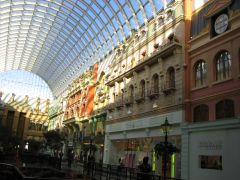
\includegraphics[width=.45\columnwidth]{Lorem}} \quad
% \subfloat[Forest landscape.]{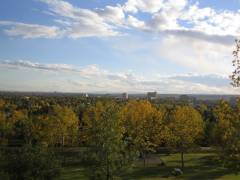
\includegraphics[width=.45\columnwidth]{Ipsum}\label{fig:ipsum}} \\
% \subfloat[Mountain landscape.]{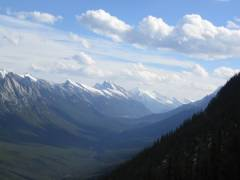
\includegraphics[width=.45\columnwidth]{Dolor}} \quad
% \subfloat[A tile decoration.]{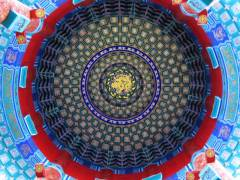
\includegraphics[width=.45\columnwidth]{Sit}}
% \caption[A number of pictures.]{A number of pictures with no common theme.} % The text in the square bracket is the caption for the list of figures while the text in the curly brackets is the figure caption
% \label{fig:esempio}
% \end{figure}

%----------------------------------------------------------------------------------------
%	BIBLIOGRAPHY
%----------------------------------------------------------------------------------------

\renewcommand{\refname}{\spacedlowsmallcaps{References}} % For modifying the bibliography heading

\bibliographystyle{unsrt}

\bibliography{sample.bib} % The file containing the bibliography

%----------------------------------------------------------------------------------------

\end{document}